\chapter{Volviendo al pasado, tercera iteración}
Continuando con el desarrollo, implementado el movimiento hacia adelante, el 
siguiente objetivo natural es ir hacia atrás.
\section{Requerimientos}
Una de las trayectorias más comunes que requiere el paciente es una simple línea
recta, de atrás hacia adelante y re regreso.
\begin{itemize}
	\item Mover el robot hacia atrás.
\end{itemize}
\section{Análisis}
Aunque la idea es simple, el cumplimiento de este objetivo nos revela grandes 
agregados a el trabajo previo:
\begin{itemize}
	\item Invertir la corriente en los motores.
	\item Añadir la funcionalidad reversa en el programa.
\end{itemize}
\section{Diseño}
Las partes implicadas son la parte eléctrica y de programación.
\subsection{Diseño electrónico}
Hasta ahora el transistor ha sido suficiente, pero ahora requiero una forma
de invertir la corriente que pasa por el motor, una forma de hacerlo es con
un circuito tipo puente, con un arreglo de seis transistores, cuatro npn y 
dos pnp, como se indica en la figura \ref{fig:puentedDc}, cuando PINB se
pone en nivel alto, provoca que Q3 y Q7 conduzcan, cuando Q3 conduce corriente, 
provoca que Q4 conduzca, con Q4 y Q7 conduciendo, la corriente puede fluir a
través del motor, si es PINA el que se enciende entonces la corriente fluye
por el motor de manera inversa, por supuesto si PINA se pone en alto
entonces PINB debe estar en bajo y viceversa, de los contrario abría un corto
circuito que probablemente dañaría los transistores.
\begin{figure}[hbt]
	\centering
	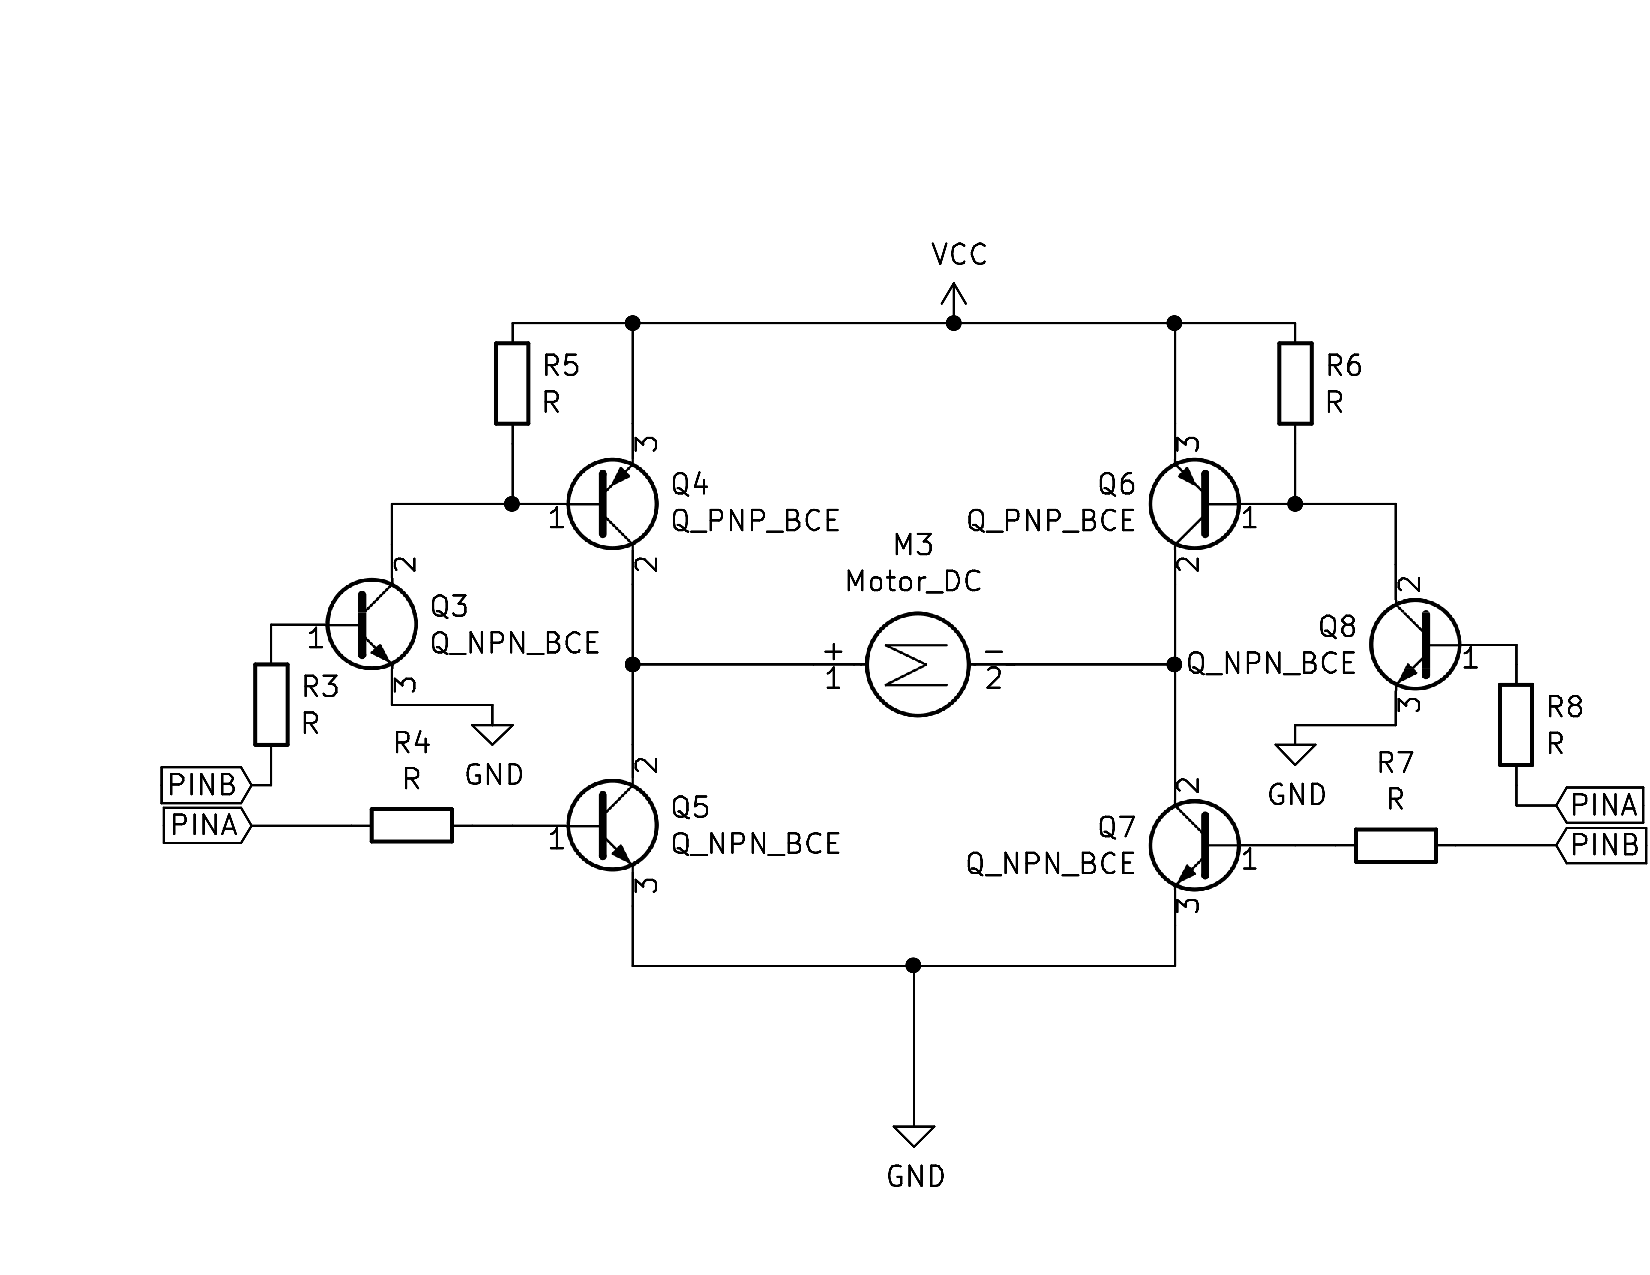
\includegraphics[page=1, width=0.9\textwidth]{it3/img/motordc.pdf}
	\caption{Puente para motor de DC}
	\label{fig:puentedDc}
\end{figure}
Sin embargo hay otra opción más simple, se puede utilizar un circuito integrado
que ya contenga esta funcionalidad, los circuitos de este tipo son llamados 
de tipo puente. Uno muy utilizado es el \emph{L298}\cite{l298}, en especifico 
este circuito integrado tiene la capacidad de manejar a dos motores, con una
potencia total de $25[W]$ y una corriente continua máxima de $2[A]$ por cada 
motor, es suficiente por ahora pero tengo mis dudas para el futuro, a ojo de 
buen cubero pienso que requiero al menos $20[W]$ por cada motor, llegado a ese 
momento decidiré que hacer con el circuito integrado.\footnote{¿Por qué no usar
un circuito integrado más poderoso de una vez?, no hay
ninguna razón técnica, es el que tengo disponible en este instante.}
Regresando al L298, 
nos permite controlar la dirección de rotación de los motores y mediante una 
técnica de conmutación también podemos controlar su velocidad. En la figura 
\ref{fig:Esquemático 3}.\footnote{El L298 requiere dos fuentes de voltaje
una para entregar potencia a los motores y otra para el control.}
\newschematic{it3/img/esquematico3.pdf}{Esquemático 3}
El circuito integrado esta dividido en dos canales A y B, uno para cada motor,
para lograr que el motor gire en la dirección que decidamos debemos establecer
las señales correspondientes a los pines de cada canal, para el canal A los pines
correspondientes son:
\begin{description}
	\item[Pin 1] Sensor de corriente, para medir la corriente del motor.
	\item[Pines 2 y 3] Salida de potencia, aquí se conectan las terminales del motor.
	\item[Pines 5 y 7] Entradas lógicas de control, estableciendo 1 y 0 respectivamente
		el motor gira a la derecha, con 0 y 1 gira en sentido contrario, 
		con 0 y 0 o con 1 y 1 el motor se detiene.
	\item[Pin 6] Habilitar, establecer un valor lógico 1, habilita la salida de 
		potencia. 
\end{description}
Por lo tanto requerimos al menos  tres pines de nuestro microcontrolador para 
controlar cada uno de los motores, tenemos muchos pines disponibles, no es un 
problema, no requerimos medir la corriente así que los pines 1 y 15 van directos
a tierra. El esquemático se ha simplificado mucho, pese a que añadí funcionalidad
estos satisfecho.
\subsection{Diseño de programa}
La arquitectura es la misma, los cambios se dan en el modulo $MotorDc$, se
requiere que cada motor utilice tres pines.
\section{Implementación}
La implementación eléctrica y mecánica como es costumbre consiste en seguir los
esquemáticos y planos, los cambios en esta etapa se dan en el software.

Modificamos la clase $MotorDc$ para contener los tres pines y para añadir un
nuevo comportamiento, ahora los motores pueden ir hacia adelante o hacia 
atrás.\footnote{Igualmente se modifican las declaraciones de los métodos virtuales
en la interfaz Motor}
\begin{minted}{C++}
class MotorDc : public Motor{
	private:
		short pin_enable_;
		short pin_input1_;
		short pin_input2_;
	public:
		MotorDc(short const pin_enable, short const pin_input1,
			       	short const pin_input2);
		virtual void forward(void) override;
		virtual void backward(void) override;
		virtual void off(void) override;
};
\end{minted}
la implementación es igualmente simple, se configuran los tres pines para indicar
el comportamiento, el código se explica por si solo.
\begin{minted}[linenos]{C++}
#include "motorDc.h"
#include "gpio.h"

MotorDc::MotorDc(short const pin_enable, short const pin_input1, short const pin_input2) :
       	pin_enable_{pin_enable}, pin_input1_{pin_input1}, pin_input2_{pin_input2}
{
	gpio_setDirection(pin_enable_, OUTPUT);
	gpio_setDirection(pin_input1_, OUTPUT);
	gpio_setDirection(pin_input2_, OUTPUT);
}
void MotorDc::forward(void)
{
	gpio_setLevel(pin_enable_, HIGH);
	gpio_setLevel(pin_input1_, HIGH);
	gpio_setLevel(pin_input2_, LOW);
}

void MotorDc::backward(void)
{
	gpio_setLevel(pin_enable_, HIGH);
	gpio_setLevel(pin_input1_, LOW);
	gpio_setLevel(pin_input2_, HIGH);
}

void MotorDc::off(void)
{
	gpio_setLevel(pin_enable_, LOW);
	gpio_setLevel(pin_input1_, LOW);
	gpio_setLevel(pin_input2_, LOW);
}
\end{minted}

Ahora que cambiamos la interfaz de $Motor$, el módulo $differential$ ya no entiende
los motores hay que modificarlo también,\footnote{Igualmente se modifica la interfaz
PowerTrain} $differential$ tiene dos funciones, las
modifico igual que $motor$,\footnote{En el futuro differential tendrá funciones
diferentes a Motor, es pura coincidencia que ahora sean iguales.} recordemos que
los motores deben girar en direcciones opuestas para hacer el desplazamiento.
\begin{minted}{C++}
#ifndef DIFFERENTIAL_H
#define DIFFERENTIAL_H

#include "power_train.h"
#include "motor.h"

class Differential : public PowerTrain{
	private:
		Motor *left_;
		Motor *rigth_;
	public:
		Differential(Motor *, Motor *);
		virtual void forward(void) override;
		virtual void backward(void) override;
		virtual void off(void) override;
};

#endif// DIFFERENTIAL_H
\end{minted}
La implementación se muestra a continuación:
\begin{minted}[linenos]{C++}
#include "differential.h"
Differential::Differential(Motor * left, Motor * right) :
       	rigth_{right}, left_{left}
{
}

void Differential::forward(void)
{
	left_->forward();
	rigth_->backward();
}

void Differential::backward(void)
{
	left_->backward();
	rigth_->forward();
}

void Differential::off(void)
{
	rigth_->off();
	left_->off();
}
\end{minted}
Invito al lector a observar lo simple y expresivo que es el código. Nuevamente 
cambiamos una interfaz, ahora todos los módulos que dependen de ella deben ser 
actualizados para que entiendan las nuevas funcionalidades, en este caso $robot$.
Actualmente robot solo tiene un método, $moveForward$, agregar $moveBackward$ es
suficiente por ahora:
\begin{minted}{C++}
#include "robot.h"

Robot::Robot(PowerTrain * train, Timer * timer):
	train_{train}, timer_{timer}
{
}
void Robot::moveForward(void)
{
	train_->forward();
	timer_->enable();
	while(timer_->getTime() < 1000);
	train_->off();
}
void Robot::moveBackward(void)
{
	train_->backward();
	timer_->enable();
	while(timer_->getTime() < 1000);
	train_->off();
}
\end{minted}
Decido extraer el botón y llevarlo a main por comodidad, el código puede 
mejorarse pero tengo la sensación de que se modificara en el siguiente hito y no
vale la pena la optimización en este instante. Finalmente el nuevo main queda así:
\begin{minted}{C++}
#include "robot.h"
#include "motorDc.h"
#include "differential.h"
#include "timer_delay.h"
#include "push.h"


int main(void)
{
	MotorDc left(9, 1, 2);
	MotorDc right(25, 23, 24);
	Differential train(&left, &right);
	Timer_delay timer;
	Robot robot(&train, &timer);
	Push push(32);

	while(1){
		if(push.pushed()){
			robot.moveForward();
			robot.moveBackward();
		}
	}
	return 0;
}
\end{minted}
\section{Pruebas}
Lo único que nos interesa es que el robot se mueva hacia atrás, puesto en marcha
observo lo siguiente.
\begin{itemize}
	\item El robot avanza y al pasar un segundo cambia bruscamente hacia 
		atrás.
	\item El freno abrupto provoca una rotación indeseable.
	\item Avanza más de lo que retrocede.
	\item Se percibe una menor potencia que cuando usaba un transistor.
\end{itemize}
Se da por cumplido el objetivo y se refinan los siguientes para corregir las 
sensaciones negativas que se han encontrado.
\section{Objetivos refinados}
\begin{itemize}
	\item Para el paciente.
		\begin{enumerate}
			\item Mover el robot de un punto A a B.
				\begin{itemize}
					\item \st{Mover hacia adelante}.
					\item \st{Mover hacia atr\'as}.
					\item Mover hacia adelante/atrás, en línea
						recta.
					\item Mover hacia adelante una x distancia.
					\item Mover hacia atrás una x distancia.
					\item Mover hacia adelante/atrás y girar hacia
						la derecha/izquierda.
					\item Girar x grados.
					\item Mover sobre una trayectoria curva.
				\end{itemize}
			\item Potencia suficiente para soportar la carga.
				\begin{itemize}
					\item Fuente de controlador.
					\item Fuente de potencia.
					\item \textbf{Selección del circuito de 
						potencia}.
					\item Tamaño y materiales de la llanta.
					\item Motores con el tamaño y torque adecuado.
					\item Acoplamiento con la base.
				\end{itemize}
			\item Movimiento save.
				\begin{itemize}
					\item Control de la velocidad.
					\item Control de la aceleración.
					\item Control diferenciado de ambos motores.
					\item Generación y seguimiento de trayectorias.
				\end{itemize}
			\item Rotación libre.
				\begin{itemize}
					\item Basé rígida y pesada.
					\item Acoplamiento encima la base.
				\end{itemize}
		\end{enumerate}
	\item Para el médico.
		\begin{enumerate}
			\item Interfaz de trayectorias.
		\end{enumerate}
	\item Para el desarrollador.
		\begin{enumerate}
			\item Dominar un nuevo lenguaje de programación.
			\item Metodologías RUP y XP.
		\end{enumerate}
\end{itemize}
